\section{第一个 CUDA 项目：核函数与执行配置}

本章将开始第一个项目——打印块和线程的 ID。这是一个非常简单的项目。从开始菜单启动 Visual Studio，创建一个新项目。在项目中
选择 CUDA 语言，然后为你的项目命名（例如 \texttt{test\_01}），点击创建。

\subsection{项目创建与核函数}

这是第一个项目，核函数文件默认为 \texttt{kernel.cu}。删除模板中的所有代码，只保留已准备好的几行头文件包含代码。本节不关注头文件部分，只关注核心代码。

假设读者已具备 C 编程语言的基础。本应用程序中有两个核函数，或者说一个核函数和一个普通函数。普通函数是主函数（\texttt{main}）——每个 C 程序都必须包含主函数，而 CUDA 代码基于 C，因此同样需要主函数。

核函数（Kernel）是将在 GPU 上执行的函数，而普通函数则在 CPU 上执行。区分两者的标志是 \texttt{\_\_global\_\_} 修饰符——带有该修饰符的即为核函数。其声明方式与普通函数类似：有返回类型、函数名、括号和大括号。当前这是一个空核函数，接下来将填充具体内容。

主函数中包含两条指令：第一条是核函数调用，第二条是 \texttt{return 0}——因为主函数类型为 \texttt{int}，所以必须返回一个整数值。

\subsection{执行配置参数}

调用核函数时，需要写出核函数名称，并配置执行参数（将影响应用程序的输出）。核函数还可以接收输入参数，例如后续章节中将对两个向量进行相加，需要在核函数中传入这些向量。本节不涉及输入参数。

本程序包含一个核函数和一个主函数，主函数调用核函数以在 GPU 上执行。

目标是打印块和线程的 ID。使用 \texttt{printf} 函数即可实现：以 \texttt{\textbackslash n} 开头换行，然后以 \texttt{\%d} 格式输出线程 ID 和块 ID，最后传入对应的变量。

CUDA 提供了预定义的块和线程索引变量：\texttt{blockIdx} 提供块 ID，\texttt{threadIdx} 提供线程 ID。CUDA 支持多维索引，本节只使用一维（\texttt{.x}）。例如，如果程序中有十个块，\texttt{blockIdx.x} 将打印从 0 到 9 的 ID。

核函数编写完成后，点击"生成（Build）"→"生成解决方案（Build Solution）"即可编译。Windows 下 Visual Studio 会自动调用 \texttt{nvcc} 编译器；Linux 用户则需要学习使用 \texttt{nvcc} 命令行编译（将在后续章节中讲解）。

核函数调用语法如下：

\texttt{核函数名<<<块数量, 每块线程数>>>();}

其中，尖括号 \texttt{<<<>>>} 内的第一个参数是网格中的块总数，第二个参数是每个块中的线程数（注意：这不是应用程序的线程总数）。当前配置为 \texttt{<<<1,1>>>}，即只有一个块、一个线程，因此输出块 ID 为 0、线程 ID 为 0。

将每块线程数增加为 4，重新构建并运行：

\begin{figure}
    \centering
    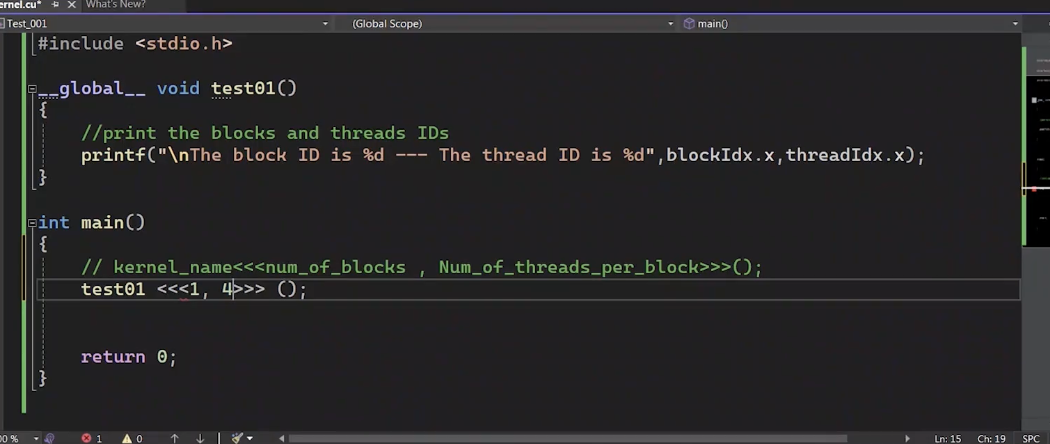
\includegraphics[width=0.75\linewidth]{resources/cuda-066.png}
    \caption{}
    \label{fig:placeholder}
\end{figure}

\subsection{逐步增加线程数与块数}

此时只有一个块，块 ID 为 0，四个线程 ID 从 0 到 3。将每块线程数增加到 32，重新构建并运行：


\begin{figure}
    \centering
    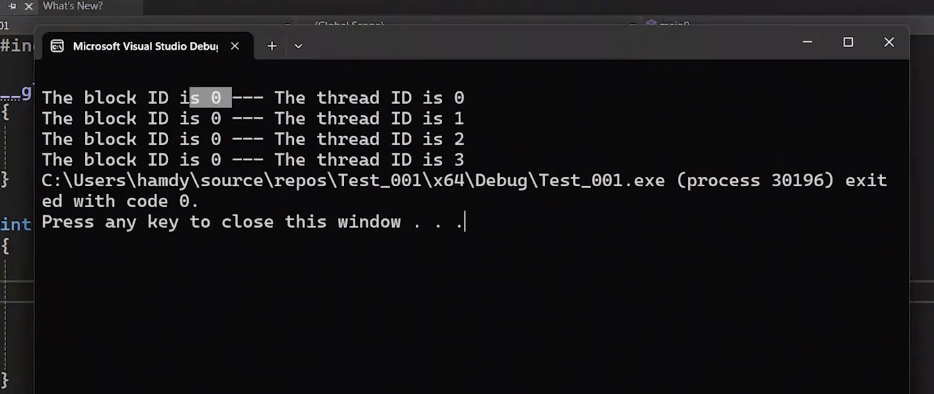
\includegraphics[width=0.75\linewidth]{resources/cuda-067.png}
    \caption{}
    \label{fig:placeholder}
\end{figure}

将块数量改为 2，每块线程数设为 8：

\begin{figure}
    \centering
    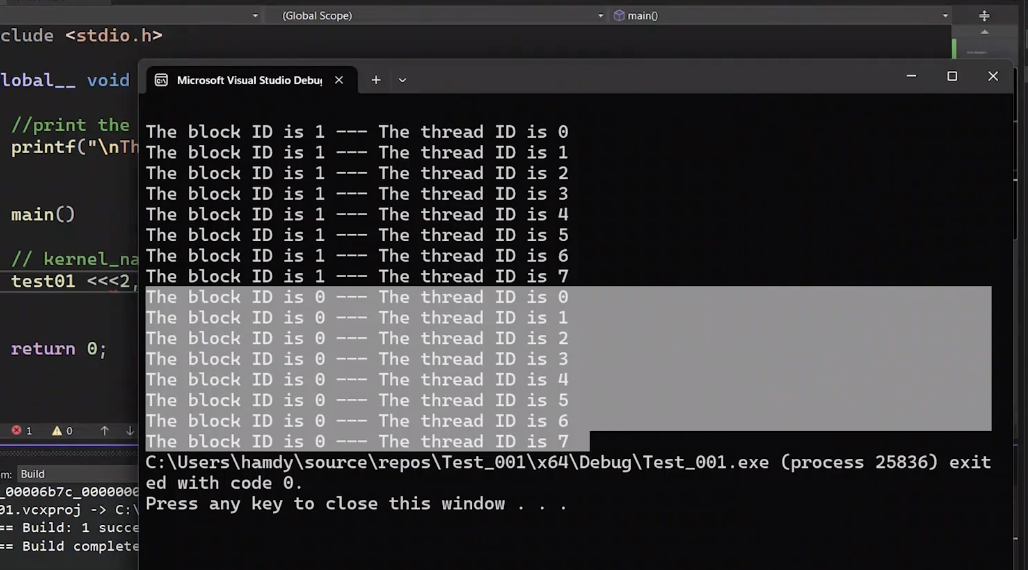
\includegraphics[width=0.75\linewidth]{resources/cuda-068.png}
    \caption{}
    \label{fig:placeholder}
\end{figure}

输出显示两个块（ID 分别为 0 和 1），每个块有 8 个线程（从 0 到 7）。你可能好奇为什么块 ID 1 先于块 ID 0 执行——这取决于哪个 SM 先接收到它的块，顺序并不重要。

接下来结合白皮书内容尝试更多配置。线程数量通常使用 2 的幂次，例如 512。将每块线程数设为 512 并运行：输出正常，块 ID 为 0，线程 ID 从 0 到 511。注意输出顺序可能不是连续的——因为线程是并行执行的，哪个线程先完成就哪个先输出，这是正常现象。

将每块线程数翻倍到 1024，运行正常，线程 ID 从 0 到 1023。再次翻倍设为 2048，运行：

\begin{figure}
    \centering
    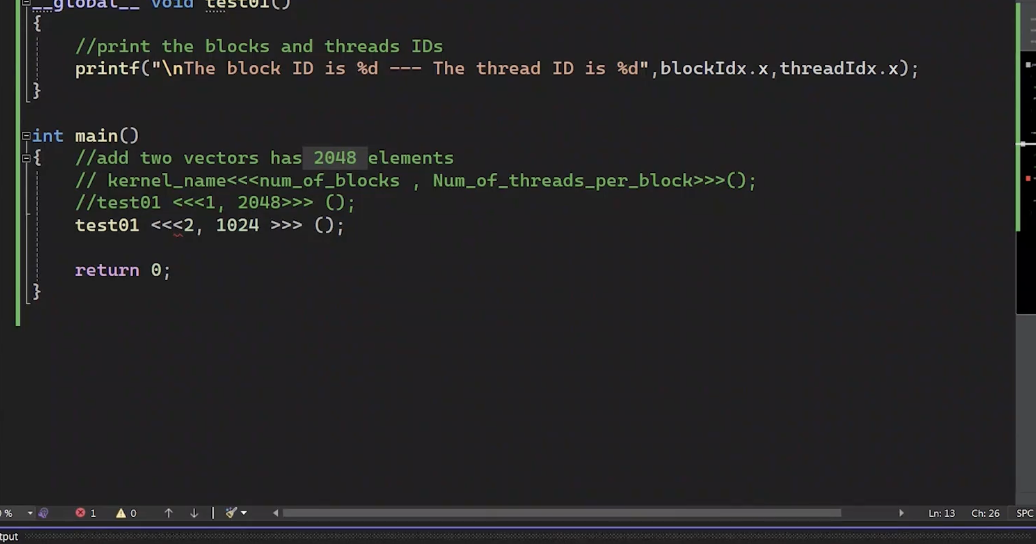
\includegraphics[width=0.75\linewidth]{resources/cuda-070.png}
    \caption{}
    \label{fig:placeholder}
\end{figure}


\subsection{硬件限制}

程序无法运行，没有任何输出。编译成功但运行失败，原因在于硬件限制。

以 Ampere 架构白皮书为例，其中的表格列出了最大线程数、最大 Warp 数、最大块数、最大寄存器数等限制。每个块的最大线程数（最大线程块大小）在 Ampere 架构中为 1024，这一限制适用于大多数架构。因此，不能将每块线程数设定为超过 1024。

这就是为什么需要同时理解软件和硬件。回到程序，假设需要对两个向量进行相加，每个向量包含 2048 个元素。如果将每块线程数设为 2048，程序将无法运行。解决方案是增加块的数量：将每块线程数设为 1024，块数设为 2（即 \texttt{<<<2, 1024>>>}），总线程数等于 $2 \times 1024 = 2048$，正好满足需求。运行后程序正常工作。

如果将块数设为 200 万，是否能运行？需要查阅白皮书中的限制。每个 SM 的最大线程块数为 32，但这是每个 SM 的限制，而非整个 GPU 的限制。整个 GPU 可运行的最大块数 = 每个 SM 最大块数 × SM 数量。例如，基于 GA100 芯片的 GPU 有 108 个 SM，因此最大并发块数为 $32 \times 108 = 3456$。

这就是软件配置与硬件限制之间的关系：每个块中的线程数与块的数量必须与硬件资源相匹配。

